\chapter{dat}

本章では、従来の辞書では指示詞を形成する語幹として挙げられている\textit{dat}に、名詞節を作る従属節標識としての用法があることを示す。さらに、意味的に似た場面で用いられる\textit{olsem}との分布の違いについても述べられる。その結果、\textit{dat}は特定の動詞の後ろに来て、文中の働きとしては直接目的語にあたる名詞節を形成する用法でのみ使用されていることが明らかになる。

\section{従来の意味}

\textit{dat}は\cite{dictionary}中に\textit{dat}単体の形で語彙として挙げられていない一方で、\textit{datfala}「その」「それ(具体的)」、\textit{datwan}「それ」という形がそれぞれ別個の指示詞として掲載されている。(\exn{1})はその\textit{datfala}の項で挙げられている例文であり
\footnote{以下、特にことわりが無ければグロスは筆者。用いる略号は基本的に\cite{prepositions}に従ったが、いくつかの必要な略号は補った: 1/2/3=1st/2nd/3rd person, SG=singular, DU=dual, PL=plural, INC=inclusive, EXC=exclusive, DEIC=deictic, PM=predicate marker, FUT=future, PERF=perfective, NEG=negative, DAT=dative, LOC=locative, POSS=possessive, TOP=topic, STATM=statement}
、ここでは\textit{datfala}が前置の修飾語として用いられているのがわかる。

\begin{exe}
  \ex
  \gll Datfala tri ia, hem long lan blong mi ia.\\
  that tree DET 3SG LOC land POSS 1SG DET\\
  \glt `That tree is on my land.'
\end{exe}

\textit{-fala}は主として形容詞接辞、\textit{-wan}は形容詞や状態動詞を名詞に変える働きを持つ接辞である\footnote{この定義は\cite{syntax}に従った。\textit{-fala}の形が定着した単語においては、直前に見た\textit{datfala}の名詞用法、三人称双数代名詞としての\textit{tufala}、一人称複数代名詞としての\textit{mifala}のように、共時的には必ずしも形容詞接辞として解釈できない意味を持つ単語もある。}一方で、徐々に多くの話者から省略されるようになってきている\citep{syntax}。
そのため、\textit{dat}単独での形でも、「その」「それ」という代名詞や限定詞としての意味を持つと推測され、事実インフォーマントへの調査においても、特定の例文を示すことなく\textit{dat}のPijin語における語義を尋ねると、この限定詞としての意味を説明されることが多かった。

\section{名詞節を形成する従属節標識として}

しかし、これから\ref{sec:datbib}節で説明するように、Pijin語聖書の中には\textit{dat}がそのままの形で現れる例が非常に多く、その意味は\textit{datfala}、\textit{datwan}として辞書に示されているような、限定詞の語幹の省略というようには解釈できない。この\textit{dat}は直後に節として解釈できる名詞・動詞などの単語が続く場合が多く、結論としては英語の\textit{that}節のように従属節標識としての機能があると考えられる。

\subsection{聖書中の用法}\label{sec:datbib}
Pijin語の新約聖書においては、\textit{dat}は単独で頻繁に登場し、その用例は全て従属節標識として解釈できる。実際の例として(\exn{1})を挙げる。\textit{dat}の後には節主語として解釈できる\textit{olketa samting ia}「この事ごと」、Pijin語を含むメラネシア・ピジン特有の述語標識\textit{i}、そして節動詞として解釈できる\textit{hapen}「起こる」と続いていて、これらの節としての意味「この事々が実際に起こったということ」が文全体の述語\textit{save}「知る」の目的語となっていることが分かる。

\begin{exe}
\ex
\gll An yufala save \underline{dat} olketa samting ya i hapen tru nao.\\
and 2PL know \underline{that} PL thing DEIC PM happen truly PERF\\
\glt `And you all know that the things really happened.' (1TH 3:4)
\end{exe}

\textit{dat}の用例は673に上り、筆者の観察ではその全てが従属節標識としての使用であった。\textit{dat}の直前の位置に来る単語の分布を表\ref{tb:datl1}に示す。

\begin{table}[h]
  \caption{dat節とその直前の位置に来る単語(1~8位)}
  \label{tb:datl1}
  \begin{minipage}{0.5\hsize}
  \begin{center}
    \begin{tabular}{|c||c|l|} \hline
      単語 & 分布数 & 対応する意味 \\ \hline \hline
      save & 168 & know\\ \hline
      somaot & 87 & show\\ \hline
      lukim & 72 & look\\ \hline
      luksave & 49 & recognise\\ \hline
    \end{tabular}
  \end{center}
  \end{minipage}
  \begin{minipage}{0.5\hsize}
    \begin{center}
      \begin{tabular}{|c||c|l|} \hline
        単語 & 分布数 & 対応する意味 \\ \hline \hline
        herem & 41 & hear \\ \hline
        talemaot & 32 & announce, reveal\\ \hline
        nao & 28 & PERF\\ \hline
        talem & 28 & tell, say\\ \hline
      \end{tabular}
    \end{center}
  \end{minipage}
\end{table}

特筆すべきことは、\textit{dat}の直前に来る単語はほとんど全てが動詞だということである。Pijin語がわりと典型的なSVO型の言語であることからも、あるいは実際の用例の観察からも、動詞の直後に来る\textit{dat}節は(\exn{0})同様に文の目的語として機能していることが分かる。表\ref{tb:datl1}の7位を占める副詞\textit{nao}は唯一動詞ではないが、この表に集計されている文章ではその全てが動詞の直後に来て完了を示す用法で使われていた\footnote{\textit{nao}は多義的な単語であり、その位置によっては全く異なる文法的意味を持つ。名詞の直後に置いてその節の話題を示したり、節の先頭につけてその節の時間的な前後関係を示す用法、あるいは文の終わりを示す用法(cf.(\ref{ex:naostatm}))が辞書\citep[145]{dictionary}には示されている。}。そして、この28例の\textit{nao dat}という単語連続は、「動詞+\textit{nao}+\textit{dat}節」というように別の動詞と\textit{dat}節の間に\textit{nao}が挿入されただけであり、\textit{dat}節自体は別の動詞の目的語としての文法的機能を担っている。実際の例として(\exn{1})を示す。ここでの\textit{dat}節は他動詞\textit{luksave}「認識する、見て分かる」の目的語となっている。

\begin{exe}
\ex
\gll ...bae olketa luksave nao \underline{dat} man ya hemi tinghae long yu.\\
FUT 3PL recognise PERF \underline{that} man DIEC 3SG-PL respect LOC 2SG\\
\glt `...then they will recognise that the man respects you.' (LUK 14:11)
\end{exe}

%このような従属節標識としての\textit{dat}の使用は、これまでPijin語について書かれてきた文法概要\cite{syntax}や辞書\cite{dictionary}、さらに現地で発行されている入門書\cite{yumi}には記載が無い一方、\cite{eric}にはごく簡単にこの用法の解説がされていた。%

\subsection{現地調査}\label{sec:datfield}

これらの聖書中の用例を踏まえ、\ref{sec:howexamined}節に述べた方法で現地での容認度調査を行った。調査は筆者が作った(\exn{1})、(\exn{2})を元にして行った。

\begin{exe}
\ex\label{dat1}
\gll Hemi talem \underline{dat} yu stap long hia.\\
3SG-PM tell \underline{that} 2SG be at here\\
\glt `He told that you are here.'
\ex\label{dat2}
\gll Mi no save \underline{dat} hem nao draev.\\
1SG NEG know \underline{that} 3SG TOP drive\\
\glt `I didn't know that he will drive.'
\end{exe}

結果、全てのインフォーマントからこの文は適格であると認められた。意味の違いについて尋ねたところ、2つの文に違いがあると述べたインフォーマントはいなかった。若い話者のほとんどは自分で話すときにも\textit{dat}を用いることがあると述べた一方で、ある50代のインフォーマント\footnote{ガダルカナル島東部のAola村の出身で、母語はLengo(オーストロネシア語族、南東ソロモン諸語)。ホニアラに来てPijinを覚えたのは30年以上前だという。}は自分以上の年代では\textit{dat}単体での使用は違和感を感じるかもしれないと答え、次のような3通りの言い方なら許されただろうと述べた。\textit{bae}は未来を示すマーカーだがPijin語にはっきりとした時制はなく\citep{eric}、未来を示す文章でも必ずしも用いる必要はない。\footnote{
  話者や文の構造による\textit{bae}(あるいは\textit{baebae}, \textit{bambae})の分布を詳細に調べた論文として\cite{bae}がある。
}。

\begin{exe}
\exi{(\exn{-1}$'$)} Hemi talem \underline{bae} yu stap long hia.
\exi{(\exn{-1}$''$)} Hemi talem \underline{dat} \underline{bae} yu stap long hia.
\exi{(\exn{-1}$'''$)} Hemi talem yu stap long hia.
\end{exe}

その後60代のインフォーマント\footnote{マライタ島南部出身で、母語はBaelelea(同じく南東ソロモン諸語)。Pijin語は第2言語として覚えたという。}に尋ねたが、彼女はこのような傾向を見せず、(\exn{-1})から(\exn{-1}$'''$)すべての文章が等しく正しいと答えた。その一方で、これらの文章はやや「宗教っぽい」響きがすると述べた。

\section{考察}
\subsection{発音}
前述した通り、\textit{dat}の従属節標識としての使用はほとんどの文法書や辞書には記載が無かったが、語学入門書である\cite{eric}には簡潔な記載がある\footnote{
\cite{eric}\vspace{0.1in}
\begin{quote}
\begin{exe}
  \exi{3.} Mi talem hem dat Bili hem i stap long Kukum. \\
  `I told him that Billy lives in Kukum.'
\end{exe}\vspace{0.1in}
Some verbs in Pijin can take \underline{\texttt{dat*}} + SENTENCE as an object instead of a simple noun phrase.
\begin{screen}
NOTE: *There are many areas in the Solomons where \underline{\texttt{dat}} is not used: Speakers who don't use \underline{\texttt{dat}} will say that the two clauses with an intonation that suggests that they are two independent sentences, or use a word borrowed from a local language.
\end{screen}
\end{quote}
}。30年以上前の記述ではあるが、この入門書によれば、本論で取り扱うような従属節標識としての用法で\textit{dat}が用いられない地域も多く、\textit{dat}を用いない話者は従属節を「2つの節が2つの独立した文であることを示すようなイントネーション」\footnote{上注の囲み部分参照。意味的にはむしろこの否定が正しいように思われるが、誤植だろうか。}によって、あるいは現地の言葉から借用した言葉によって話すと述べられている。

今回の都市部における調査では、そもそも\textit{dat}を許容しない話者を見つけられなかったため、後者の現地からの借用語については確認することができなかったが、前者のイントネーションについてはある程度確認できたため、非常に粗縛な形ではあるがここに分析する。\cite{eric}の記述によれば、通常の叙述文の一般的なイントネーションのパターンは図\ref{fig:intonation}のような形を取る。文は中間くらいの高さ(2)で比較的平坦に話され、文の最後となる強勢で上がり(3)、それから低く落ちる(1)。

\begin{figure}[ht]
  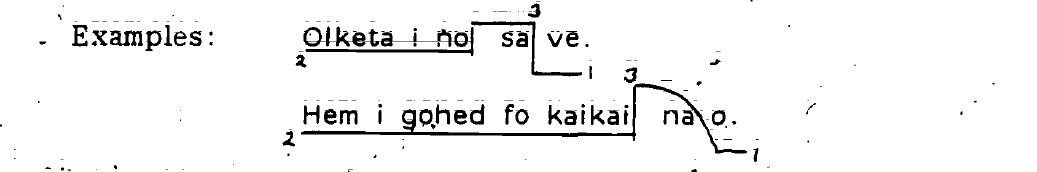
\includegraphics[width=15cm]{./intonation.png}
  \caption{Pijin語叙述文における一般的なイントネーションのパターン\cite[10]{eric}}
  \label{fig:intonation}
\end{figure}

今回筆者が録音した用例を聞く限りでは、\textit{dat}を用いずに動詞の目的語として節を取る発話では(a)速い発話では、動詞に続いて間を置かずに話される (b)ゆっくりの発話では、文が続くことを示すために動詞の語尾が下降しない という特徴があるように感じられた。いずれの場合においても、イントネーションは2つの節(主節、従属節)がバラバラの2つの文ではなく、全体で1つの文であるということを考えれば、図\ref{fig:intonation}のパターンに合致しているように思われる。通常文が終わるタイミングではイントネーションが下降するため、ゆっくりの発音でもその下降がなければ聞き手に一文がまだ続いているという情報を伝えることができる。しかし、このイントネーションが\cite{eric}によって示されたものと同一であるかどうかには疑念がある。

\cite{phonology}はPijin語についてのイントネーションに対する包括的な記述はまだ無いと記した上で、イントネーションがPijin語の文の意味解釈に与える影響の大きさについて記している。その一方で将来のPijin語について、「ことによると文法化の進行は情報伝達におけるイントネーションの必要性を減少させるかもしれず、言語がより成熟しより標準化していく中で、ことによるとイントネーションの使用は文法的標識に役割を譲り、音韻はより規則に従ったものになるかもしれない」\footnote{``Perhaps increasing grammaticalization will reduce the need for intonation in conveying information and, as the language gets older and more standardized, perhaps the use of intonation will give way to grammatical markers, and the phonology will become more regular.''\citep{phonology}}とも述べている。\textit{dat}という従属節標識の(部分的な)導入とこの節で示したイントネーションとの関係は、まさにここで示されているような現象の1つかもしれない。

\subsection{英語のthat節との比較}

ここで取り上げたような\textit{dat}の従属節標識としての使用は、その発音からも用法からも英語の\textit{that}節からある程度の影響があったということは否定できないだろう。一方で、これから検証していくように、少なくとも聖書の中での用法は英語と比較して限定的であり、借用はある程度限定的である。

まず、英語の\textit{that}節には制限用法に限って関係節標識としての用法が存在する\cite[365-367]{english}が、Pijin語の\textit{dat}には見当たらない。\cite{dictionary}には関係節標識として\textit{we}と\textit{hu}が挙げられているが、聖書の場合も同様の用法で\textit{wea}と\textit{hu}を利用している。

さらに、名詞従属節標識としての機能も、英語に比べるとかなり限られている。\cite{english}は文中の英語\textit{that}節の用法として次の5つを挙げている。

\begin{enumerate}
  \item 主語 : \textit{That the invading troops have been withdrawn} has not affected our government's trade sanctions.
  \item 直接目的語 : I noticed \textit{that he spoke English with an Australian accent}.
  \item 主格補語 : My assumption is \textit{that interest rates will soon fall}.
  \item 同格 : Your criticism, \textit{that no account has been taken of psychological factors}, is fully justified.
  \item 形容詞補語 : We are glad \textit{that you are able to join us on our wedding anniversary}.
\end{enumerate}

Pijin語における\textit{dat}節の働きは、聖書で筆者が観察した限りでは(b)すなわち直接目的語としての用法に限られていて、それ以外の用法は別の従属節標識が担っているように思われる。すなわち、(a)(c)(d)は次節で取り上げる\textit{olsem}が、(e)は次章で取り上げる\textit{fo}が用いられているのである。\cite{english}は主語の後置(\textit{it is that...})という形を(a)の際によく起こる現象として記しているが、これはPijin語では(\exn{1})のような\textit{hemi olsem...}あるいは\textit{hem nao olsem...}という形をとり、やはり\textit{dat}は使われない。

\begin{exe}
  \ex
  \gll Hemi \underline{olsem} yumi lukim long glas wea hemi no klia gudfala.\\
  3SG-PM \underline{like} 1PL.INC look LOC glasses REL 3SG-PM NEG clear well\\
  \glt ``It is like that we are looking at a glass which is not clear enough.'' (1CO 13:13)
\end{exe}

\subsection{olsem節との使い分け}
\textit{olsem}は\cite{dictionary}では「~のような(like that, as if)」という意味のみが示されている。従属節標識としての例文は(\exn{1})が挙げられているが、ここでの意味も同様に解釈できる。

\begin{exe}
  \ex\label{ex:naostatm}
  \gll Man toktok \underline{olsem} hem bikman nao.\\
  man talk \underline{like} 3SG important-man STATM\\
  \glt ``This man talks as if he were an important man.'' \citep[157]{dictionary}
\end{exe}
